

\section{MetaPreprocess}

In this section, we introduce how to upload your datasets into the MetaOmics software suite such that each functional modules can be utilized.
The R package for MetaPreprocess module can be found \url{https://github.com/metaOmics/preproc}.

\subsection{Procedure}
\label{sec:procedure}

\begin{steps}
\item \textbf{Uploading data:}

\begin{figure}[!htbp]
\begin{center}
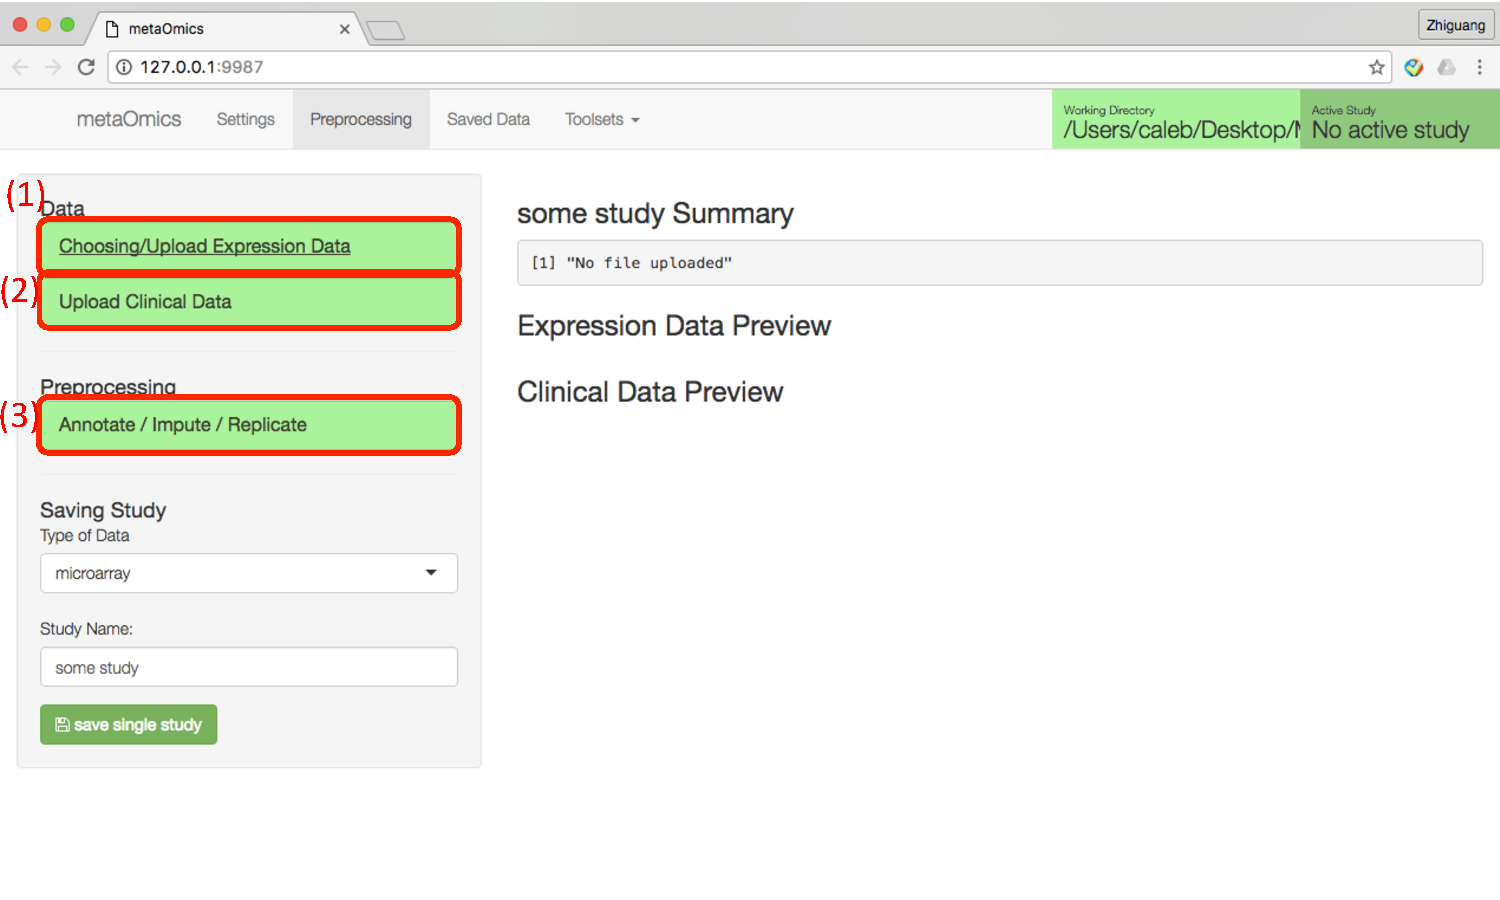
\includegraphics[scale=0.7]{./figure/preprocessing/GUIpreprocessing}
\caption{GUI Preprocessing page}
\label{fig:GUIpreprocessing}
\end{center}
\end{figure}

After clicking the Preprocessing tab as on top of Figure~\ref{fig:GUIpreprocessing},
users can click on ``Choosing/Upload Expression Data" tab to upload individual expression data files or choose the existing saved data file as in Figure~\ref{fig:GUIpreview} (at position {\color{red} (1)}).
The data should be prepared according to Section~\ref{sec:dataPrepare}.
Users may optionally upload Clinical Data (at position {\color{red} (2)}), depending on their biological purposes.
All MetaOmics modules except for MetaClust  require external clinical labels.
Three example datasets are available within MetaOmics folder ``metaOmics/data/example/",
but we will focus on the leukemia dataset (``metaOmics/data/example/") throughout this tutorial.

\item \textbf{Preprocessing:}

The MetaOmics suit also provides handlers (at position {\color{red} (3)} of Figure~\ref{fig:GUIpreprocessing}) for feature annotation, missing value imputation and multiple probe same genes.
After the csv file for gene expression profile is specified, 
users can preview their data on the right hand side of the page as Figure~\ref{fig:GUIpreview}.
Several expression data parsing options (e.g. header, column separator, etc) are available on the left panel of Figure~\ref{fig:GUIpreview}.
For preprocessing, 
click on ``Annotate/Impute/Replicate" to 
\begin{enumerate}
\item annotate the probe ID/reference sequence ID/Entrez ID of individual dataset (choose Gene Symbol if the input data rows are already annotated).
\item impute missing value using knn method.
\item handle the multiple probes matching to the same gene issue.
\end{enumerate}

A complete introduction of these options is available at the end of this subsection.
The right hand side of Figure~\ref{fig:GUIpreview} shows the summary statistics of uploaded data and preview of the data matrix.
There is a search box such that the users can search their favorite genes.

\begin{figure}[H]
\begin{center}
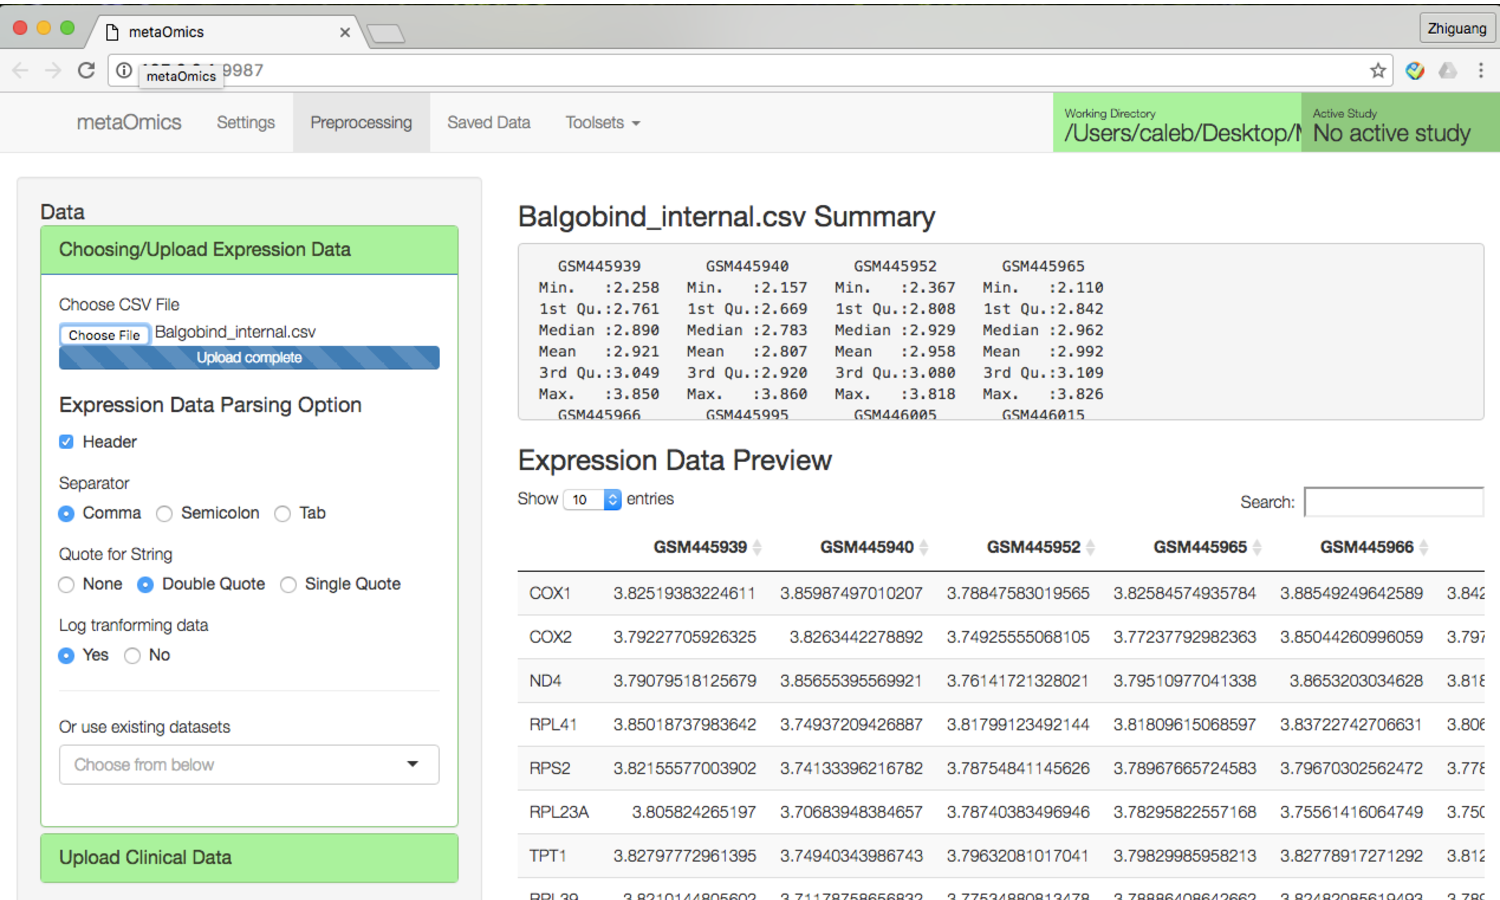
\includegraphics[scale=0.7]{./figure/preprocessing/GUIpreview}
\caption{Uploading individual studies}
\label{fig:GUIpreview}
\end{center}
\end{figure}

\item \textbf{Save single study:}
In the next step,
specify the data type (``microarray" or ``RNA-seq", continuous or discreate) and study name,
click ``save single study".
To upload RNA-seq data, the count data file and FPKM/TPM
 data should be uploaded separately and saved using different names.

\item \textbf{Upload datasets for all studies:}
Repeat the steps above for all studies for meta-analysis.
All uploaded studies are now available in the ``Saved Data" tab. 
 
\end{steps}

\subsection{Saved Data tab}
\label{sec:saved}

After uploading multiple studies with or without clinical data,
users can turn to the Saved Data tab.

\begin{figure}[H]
\begin{center}
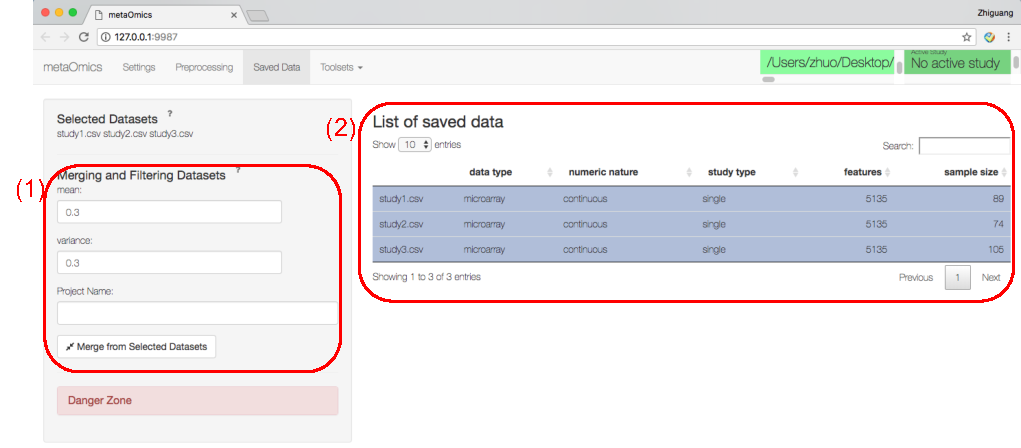
\includegraphics[scale=0.9]{./figure/preprocessing/GUImerge.pdf}
\caption{Merge from selected datasets}
\label{fig:GUImerge}
\end{center}
\end{figure}


\begin{steps}
\item \textbf{Merging and Filtering:}
All saved datasets from the previous step will be found in  Figure~\ref{fig:GUImerge} (at position {\color{red} (2)}).
Users should select multiple datasets for further meta-analysis purpose.
Users can filter out genes with low expression level (by default, mean expression lower than $30^{th}$ percentile)
or low variance (by default, variance lower than $30^{th}$ percentile).
Low expression genes can be non-expressed genes and low variance genes can be non-informative genes thus including them may contribute false positives.
After specifying filtering criteria, enter Project Name and click on the ``Merge from Selected Datasets" (at position {\color{red} (1)}).
A merged dataset (study type = ``multiple") will appear on the  ``List of saved data" panel (at position {\color{red} (3)}).
Creating multiple projects with varying preprocessing criteria is useful.
For example, the user can start from a project with harsh filtering criteria (maintain 500-1000 genes) and give a test run through all modules to save time.
If successful, a larger project can be created and implemented.
If users want to delete any dataset, they can click the red danger zone button and delete selected dataset.

\item \textbf{Make active dataset:}
\label{sec:active}
The last thing to do before using meta-analytic toolsets is to select merged data and click on 
``Make your dataset Active Dataset" - A big green button in Figure~\ref{fig:active}.
Then the merged data becomes active study and shows up on the top right corner.
The active dataset serves as the input for all other MetaOmics modules.


\end{steps}







\begin{figure}[H]
\begin{center}
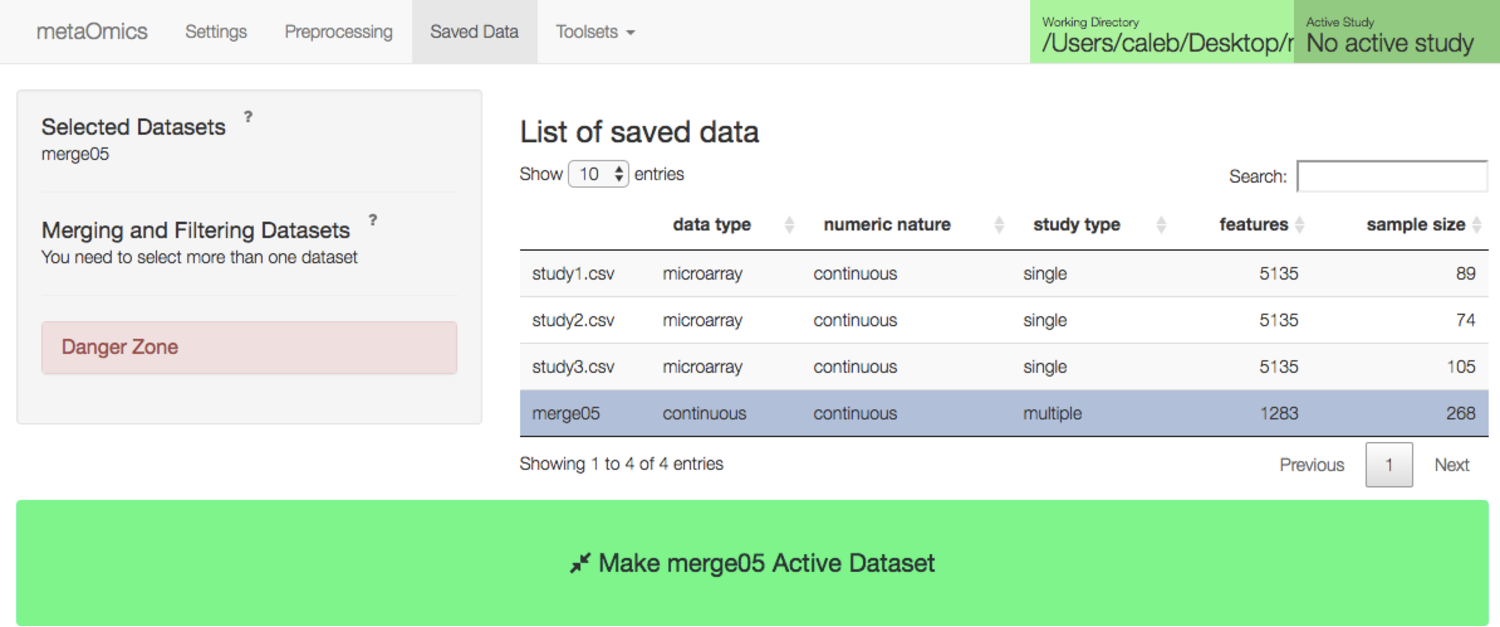
\includegraphics[scale=0.7]{./figure/preprocessing/GUImarkActive}
\caption{Make merged Dataset Active}
\label{fig:active}
\end{center}
\end{figure}




\textbf{Complete List of Options:} 
\begin{enumerate}
\item Upload expression data:
\begin{itemize}
\item Header: should be checked if the input file includes a header.
\item Separator: indicates what type of separator is used for the data matrix.
\item Quote for String: how is the data matrix quoted.
\item Log transforming data: if you want to perform log transformation of your data, check yes.
\item Use existing datasets: if you want to load a dataset previously uploaded, you can choose from the checklist.
\end{itemize}
\item Annotation/impute/Replicate:
\begin{itemize}
\item Annotation: possible ID type can be Gene Symbol (default), Probe ID, reference sequence ID, entrez ID.
\item Impute: if selected, missing value imputation will be performed by k-nearest neighbor algorithm.
\item Replicate Handling: if selected, if the same gene symbol maps to multiple probes, the probe with the largest inner quantile range (IQR) will be selected
as a representative for this gene.
\end{itemize}
\item Saved Data, Merging and Filtering Datasets:
\begin{itemize}
\item Mean: the criteria such that how many percent of genes will be filtered out based on sum of mean ranks (e.g. 0.3 represent 30\%).
\item Variance: after the Mean filtering, the criteria such that how many percent of genes will be filtered out based on sum of variance ranks (e.g. 0.3 represent 30\%).
\item Study Name: dataset name after merging. This name will appear in the list of saved data table.
\item Merge from Selected Datasets: perform filtering and merging.
\end{itemize}
\item Danger zone:
\begin{itemize}
\item Delete Selected Data: the selected data will be delete permanently if clicked, so please be cautious.
\end{itemize}

\end{enumerate}



